%%%%%%%%%%%%%%%%%%%%%%%%%%%%%%%%%%%%%%%%%%%%%%%%%%%%%%%%%%%%%%%%%%
%
% Analysis of Algorithms
%
% Homework Assignment #5
%
%%%%%%%%%%%%%%%%%%%%%%%%%%%%%%%%%%%%%%%%%%%%%%%%%%%%%%%%%%%%%%%%%%
%%%%%%%%%%%%%%%%%%%%%%%%%%%%%%%%%%%%%%%%%%%%%%%%%%%%%%%%%%%%%%%%%%
%
% Score Card and Answer Sheets
%
%%%%%%%%%%%%%%%%%%%%%%%%%%%%%%%%%%%%%%%%%%%%%%%%%%%%%%%%%%%%%%%%%%
\documentclass[addpoints,11pt]{exam}
\usepackage{clrscode3e}
\usepackage{commath}
\usepackage{units}
\usepackage{enumitem}
\usepackage{fullpage}
\usepackage[usenames,dvipsnames]{xcolor}
\usepackage{amsmath}
\usepackage{amstext}
\usepackage{pdfpages}
\usepackage{tikz}
\usepackage{verbatim}
\usetikzlibrary{arrows,shapes}
\usepackage{tikz-qtree}
\usepackage{booktabs}
\usepackage{float}
\usepackage{grffile}
\usepackage{graphicx}
\usepackage{forest}
\usepackage{tkz-graph}
\usepackage{minted}


%%%%%%%%%%%%%%%%%%%%%%%%%%%%%%%%%%%%%%%%%%%%%%%%%%%%%%%%%%%%%%%%%%
%
% Begin Document
%
%%%%%%%%%%%%%%%%%%%%%%%%%%%%%%%%%%%%%%%%%%%%%%%%%%%%%%%%%%%%%%%%%%
\begin{document}
\pagestyle{empty}


\noindent{\large\bfseries Name: \hrulefill John Henry Mejia}\\
\noindent{\large\bfseries COSC 40403 - Analysis of Algorithms: Homework 5}\\



%%%%%%%%%%%%%%%%%%%%%%%%%%%%%%%%%%%%%%%%%%%%%%%%%%%%%%%%%%%%%%%%%%
%
% Score Card and Answer Sheets
%
% Comment out one-or-the-other to show or not-show the answers.
%
%%%%%%%%%%%%%%%%%%%%%%%%%%%%%%%%%%%%%%%%%%%%%%%%%%%%%%%%%%%%%%%%%%
%\SolutionEmphasis{\color{Blue}}
\renewcommand{\solutiontitle}{\noindent\textbf{Answer:}\par\noindent}
\printanswers
%\noprintanswers


%%%%%%%%%%%%%%%%%%%%%%%%%%%%%%%%%%%%%%%%%%%%%%%%%%%%%%%%%%%%%%%%%%
% Begin Questions
%%%%%%%%%%%%%%%%%%%%%%%%%%%%%%%%%%%%%%%%%%%%%%%%%%%%%%%%%%%%%%%%%%
\begin{questions}



%%%%%%%%%%%%%%%%%%%%%%%%%%%%%%%%%%%%%%%%%%%%%%%%%%%%%%%%%%%%%%%%%%
% Question
%%%%%%%%%%%%%%%%%%%%%%%%%%%%%%%%%%%%%%%%%%%%%%%%%%%%%%%%%%%%%%%%%%
\question [10] Show (prove) that the greedy approach always fins an optimal solution for the Make-Change problem when the coins are in the denominations $D^0$, $D^1$, $D^2$, \dots, $D^i$ for some integers $i>0$ and $D>0$.

\begin{solutionorbox}

   

    Let $a_0 \cdot D^0$, $a_1 \cdot D^1$, $a_2 \cdot D^2$, \dots, $a_i \cdot D^i$ represent an greedy solution.

    First note that $a_j < D$ for all $j < i$ in the greedy algorithm. This is merely because we could replace D coins of denomination $D^j$ with a single coin of the demonic denomination that is $D^j+1$ if it wasn't the case that $a_j < D$ for all $j < i$. 

    Now let $a_i$ suppose the number of coins used in a optimal solution for making change of n cents. 

    Let us suppose that such an algorithm is not greedy for the sake of argument by contradiction: then for one coin $a_j$ it is not the same as in the greedy algorithm. Let us suppose we are talking about the greatest coin $D^i$ that differs from the greedy algorithm, then we know that the coin $a_i$ in this "non-greedy-optimal algorithm" MUST be less than the one selected by the greedy algorithm. This is because the greedy algorithm already has the maximum amount of coins. (having 1 more would make the value too high.)

    By having less coins than before, then we would increase older values $a_{i-1}$ by a value of D. This would not be optimal because as shown above if any coin $D^m$ has a value over D we can simply increase the coin $D^m+1$ to find a solution with less coins. 

    Therefore the optimal solution for all i is the greedy solution.

   Since for all i the greedy solution is the optimal solution this means that the greedy algorithm IS the optimal algorithm. 
    
\end{solutionorbox}

\ifprintanswers
\newpage
\else
\bigskip
\fi


%%%%%%%%%%%%%%%%%%%%%%%%%%%%%%%%%%%%%%%%%%%%%%%%%%%%%%%%%%%%%%%%%%
% Question
%%%%%%%%%%%%%%%%%%%%%%%%%%%%%%%%%%%%%%%%%%%%%%%%%%%%%%%%%%%%%%%%%%
\question (\totalpoints \text{ points total}) Answer the following questions regarding Huffman's algorithm.
\begin{parts}
	\part [5] Use Huffman's algorithm to construct an optimal binary prefix code for the letters in the following table.  Note: if two sub-trees have the same value, the sub-tree with more nodes has priority.  Show your work.\\
	
	\begin{tabular}{|l|l|l|l|l|l|l|l|}
		\hline
		\textit{\textbf{LETTER}}    & T  & U & V  & W  & X & Y & Z \\ \hline
		\textit{\textbf{FREQUENCY}} & 12 & 7 & 18 & 10 & 9 & 5 & 2 \\ \hline
	\end{tabular}\\
	\part [5] Decode each bit string using your binary code.  Note: there may be left-over bits that cannot be decoded.  Show your work.
	\begin{enumerate} [label=(\roman*.)]
		\item {\tt 01010101000110}
		\item {\tt 0101001000100}
		\item {\tt 11001110001111}
		\item {\tt 0011101000010}
	\end{enumerate}
\end{parts}

\begin{solutionorbox}
    \begin{parts}
        \part  Remember, to create a Huffman tree we must start by making each unique character and their value within a min heap. So we start with Z at the top of the min heap. We then extract the min heap Z (2) and reheapify, so that the next lowest is Y. We then combine these 2 and start building our Huffman tree. 

        Now the value of ZY is 7. Both U and ZY have a value of 7 but since the subtree with more nodes has priority, ZY has priority. Therefore it is the lowest on the min heap and so we end up combining them into the following tree: 
        
\begin{forest}
for tree={
    rounded corners, draw, align=center, top color=white, bottom color=blue!20,
    edge+=->,
    l sep'+=10pt,
}
[14, edge label={node[midway,right] {1}}, red
[7, edge label={node[midway,left] {0}},red 
    [2(Z), edge label={node[midway,left] {0}} ]
    [5(Y), edge label={node[midway,right] {1}}]
]
[U(7), edge label={node[midway,right] {1}}]
]
\end{forest}

We then reheapify and consider the next lowest value, X. X is not connected to ZYU and so it is part of its own tree right now: 

\begin{forest}
for tree={
    rounded corners, draw, align=center, top color=white, bottom color=blue!20,
    edge+=->,
    l sep'+=10pt,
}
[, phantom, s sep = 1cm
[14, edge label={node[midway,right] {1}}, red
[7, edge label={node[midway,left] {0}},red 
    [2(Z), edge label={node[midway,left] {0}} ]
    [5(Y), edge label={node[midway,right] {1}}]
]
[U(7), edge label={node[midway,right] {1}}]
]
[9(X), edge label={node[midway,left] {0}} ]
]
\end{forest}


We then take 10, which is the next lowest, making XW into one with the value of 19. We then take 12 (T) and combine that with 14  (ZYU) and making a value of 26.

\begin{forest}
for tree={
    rounded corners, draw, align=center, top color=white, bottom color=blue!20,
    edge+=->,
    l sep'+=10pt,
}
[, phantom, s sep = 1cm
[26, edge label={node[midway,left] {0}}, red 
      [12(T), edge label={node[midway,left] {0}} ]
      [14, edge label={node[midway,right] {1}}, red
[7, edge label={node[midway,left] {0}},red 
    [2(Z), edge label={node[midway,left] {0}} ]
    [5(Y), edge label={node[midway,right] {1}}]
]
[U(7), edge label={node[midway,right] {1}}]
      ]
    ]
[19, edge label={node[midway,right] {1}}, red
        [9(X), edge label={node[midway,left] {0}} ]
        [10(W), edge label={node[midway,right] {1}} ]
      ] 
]
\end{forest}

Next, we take 18, combine with 19 to make a value of 3. We Finally take 26 (ZYUT) and combine with 37 (XVW) to create our final huffman tree:

\begin{forest}
for tree={
    rounded corners, draw, align=center, top color=white, bottom color=blue!20,
    edge+=->,
    l sep'+=10pt,
  }
[63,red 
    [26, edge label={node[midway,left] {0}}, red 
      [12(T), edge label={node[midway,left] {0}} ]
      [14, edge label={node[midway,right] {1}}, red
[7, edge label={node[midway,left] {0}},red 
    [2(Z), edge label={node[midway,left] {0}} ]
    [5(Y), edge label={node[midway,right] {1}}]
]
[U(7), edge label={node[midway,right] {1}}]
      ]
    ]
    [37, edge label={node[midway,right] {1}}, red
      [18(V), edge label={node[midway,left] {0}} ] 
      [19, edge label={node[midway,right] {1}}, red
        [9(X), edge label={node[midway,left] {0}} ]
        [10(W), edge label={node[midway,right] {1}} ]
      ] 
  ] 
]
\end{forest}
        \part  \begin{enumerate} [label=(\roman*.)]
		\item {\tt 0101 0101 00 011 0} \break
            The first item we take is Y (0101) and then Y (0101) and then T (00) and then U (011)

            So YYTU 0
            
		\item {\tt 0101 00 10 00 10 0} \break
            It is therefore imperative to the continuing success of lossless compression algorithms for such importance to be known. 

            Y T V T V 0 
		\item {\tt 110 011 10 00 111 1}
  
            X U V T W 1
		\item {\tt 00 111 0100 00 10}
  
        T W Z T V
	\end{enumerate}
            
    \end{parts}
\end{solutionorbox}

\ifprintanswers
\newpage
\else
\bigskip
\fi

	
%%%%%%%%%%%%%%%%%%%%%%%%%%%%%%%%%%%%%%%%%%%%%%%%%%%%%%%%%%%%%%%%%%
% Question
%%%%%%%%%%%%%%%%%%%%%%%%%%%%%%%%%%%%%%%%%%%%%%%%%%%%%%%%%%%%%%%%%%
\question[10]
Use Prim's algorithm to find a minimum spanning tree for the following graph.  Show the actions step by step.

\includegraphics[scale=0.5]{g1a.pdf}
\begin{solutionorbox}


\begin{tikzpicture}
    \GraphInit[vstyle=Dijkstra]
    \SetGraphUnit{4}
    \Vertex{v1}
    \EA(v1){v2}
    \SO(v1){v4}
    \SO(v2){v5}
    \EA(v5){v6}
    \SO(v6){v10}
    \SO(v5){v9}
    \SO(v4){v8}
    \WE(v4){v3}
    \SO(v3){v7}
    
    \Edge[label=$32$](v1)(v2)
    \Edge[label=$17$](v1)(v4)
    \Edge[label=$45$](v2)(v5)
    \Edge[label=$18$](v3)(v4)
    \Edge[label=$10$](v4)(v5)
    \Edge[label=$28$](v6)(v5)
    \Edge[label=$5$](v3)(v7)
    \Edge[label=$3$](v4)(v8)
    \Edge[label=$25$](v5)(v9)
    \Edge[label=$6$](v6)(v10)
    \Edge[label=$59$](v7)(v8)
    \Edge[label=$4$](v8)(v9)
    \Edge[label=$12$](v9)(v10)
    \SetUpEdge[lw=4pt,color=red]
    
\end{tikzpicture}


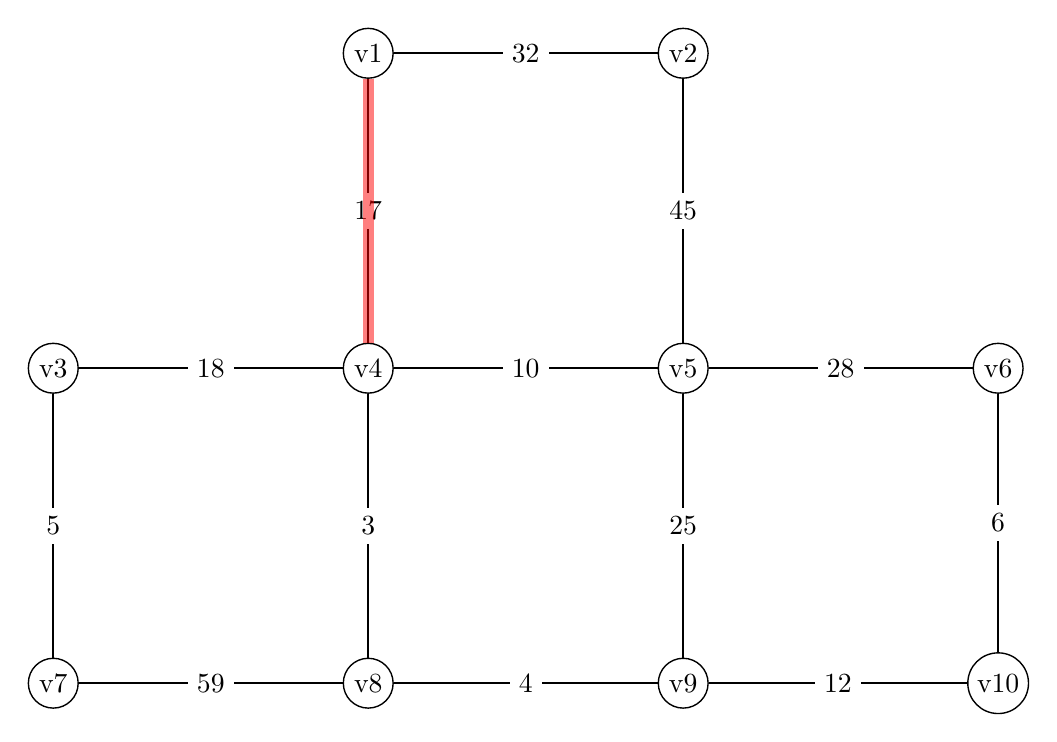
\begin{tikzpicture}
    \GraphInit[vstyle=Dijkstra]
    \SetGraphUnit{4}
    \Vertex{v1}
    \EA(v1){v2}
    \SO(v1){v4}
    \SO(v2){v5}
    \EA(v5){v6}
    \SO(v6){v10}
    \SO(v5){v9}
    \SO(v4){v8}
    \WE(v4){v3}
    \SO(v3){v7}
    
    \Edge[label=$32$](v1)(v2)
    \Edge[label=$17$](v1)(v4)
    \Edge[label=$45$](v2)(v5)
    \Edge[label=$18$](v3)(v4)
    \Edge[label=$10$](v4)(v5)
    \Edge[label=$28$](v6)(v5)
    \Edge[label=$5$](v3)(v7)
    \Edge[label=$3$](v4)(v8)
    \Edge[label=$25$](v5)(v9)
    \Edge[label=$6$](v6)(v10)
    \Edge[label=$59$](v7)(v8)
    \Edge[label=$4$](v8)(v9)
    \Edge[label=$12$](v9)(v10)
    \SetUpEdge[lw=4pt,color=red]
    \Edges[style={opacity=.5}](v1,v4)
\end{tikzpicture}

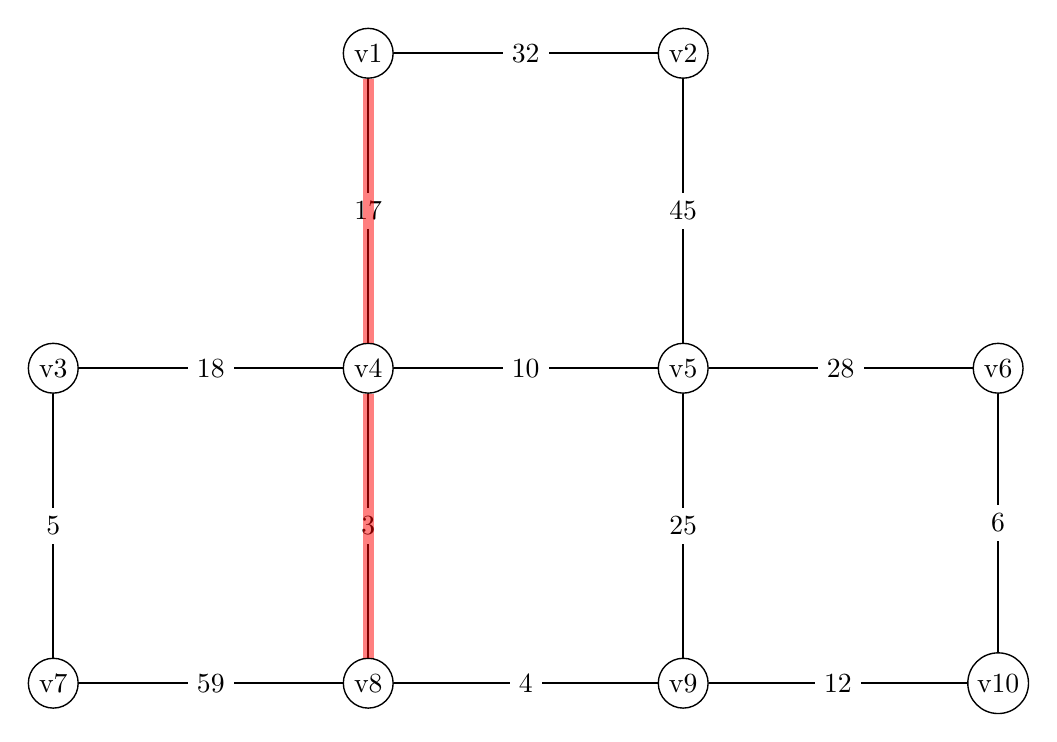
\begin{tikzpicture}
    \GraphInit[vstyle=Dijkstra]
    \SetGraphUnit{4}
    \Vertex{v1}
    \EA(v1){v2}
    \SO(v1){v4}
    \SO(v2){v5}
    \EA(v5){v6}
    \SO(v6){v10}
    \SO(v5){v9}
    \SO(v4){v8}
    \WE(v4){v3}
    \SO(v3){v7}
    
    \Edge[label=$32$](v1)(v2)
    \Edge[label=$17$](v1)(v4)
    \Edge[label=$45$](v2)(v5)
    \Edge[label=$18$](v3)(v4)
    \Edge[label=$10$](v4)(v5)
    \Edge[label=$28$](v6)(v5)
    \Edge[label=$5$](v3)(v7)
    \Edge[label=$3$](v4)(v8)
    \Edge[label=$25$](v5)(v9)
    \Edge[label=$6$](v6)(v10)
    \Edge[label=$59$](v7)(v8)
    \Edge[label=$4$](v8)(v9)
    \Edge[label=$12$](v9)(v10)
    \SetUpEdge[lw=4pt,color=red]
    \Edges[style={opacity=.5}](v1,v4)
    \Edges[style={opacity=.5}](v4,v8)
\end{tikzpicture}

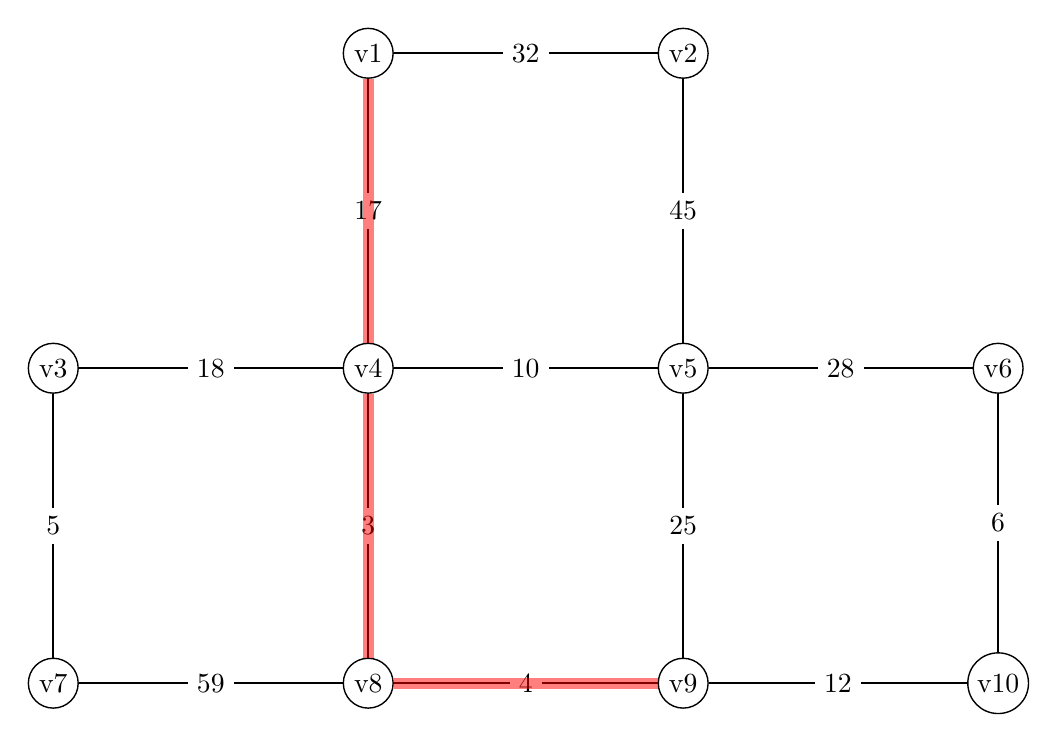
\begin{tikzpicture}
    \GraphInit[vstyle=Dijkstra]
    \SetGraphUnit{4}
    \Vertex{v1}
    \EA(v1){v2}
    \SO(v1){v4}
    \SO(v2){v5}
    \EA(v5){v6}
    \SO(v6){v10}
    \SO(v5){v9}
    \SO(v4){v8}
    \WE(v4){v3}
    \SO(v3){v7}
    
    \Edge[label=$32$](v1)(v2)
    \Edge[label=$17$](v1)(v4)
    \Edge[label=$45$](v2)(v5)
    \Edge[label=$18$](v3)(v4)
    \Edge[label=$10$](v4)(v5)
    \Edge[label=$28$](v6)(v5)
    \Edge[label=$5$](v3)(v7)
    \Edge[label=$3$](v4)(v8)
    \Edge[label=$25$](v5)(v9)
    \Edge[label=$6$](v6)(v10)
    \Edge[label=$59$](v7)(v8)
    \Edge[label=$4$](v8)(v9)
    \Edge[label=$12$](v9)(v10)
    \SetUpEdge[lw=4pt,color=red]
    \Edges[style={opacity=.5}](v1,v4)
    \Edges[style={opacity=.5}](v4,v8)
    \Edges[style={opacity=.5}](v8,v9)
\end{tikzpicture}

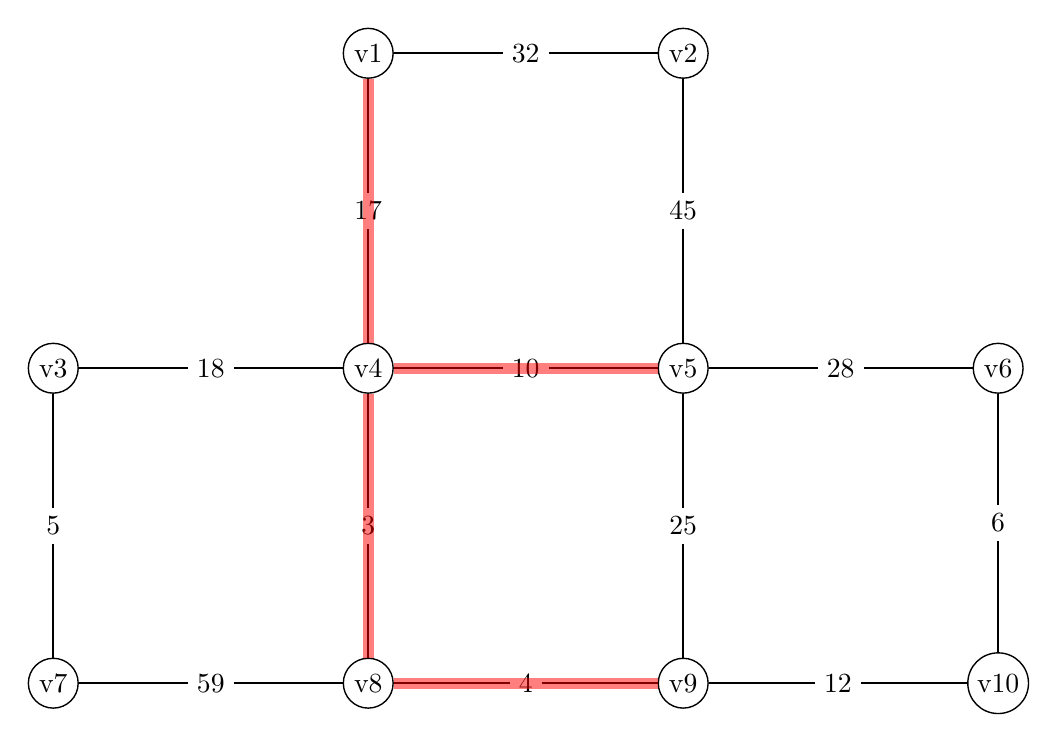
\begin{tikzpicture}
    \GraphInit[vstyle=Dijkstra]
    \SetGraphUnit{4}
    \Vertex{v1}
    \EA(v1){v2}
    \SO(v1){v4}
    \SO(v2){v5}
    \EA(v5){v6}
    \SO(v6){v10}
    \SO(v5){v9}
    \SO(v4){v8}
    \WE(v4){v3}
    \SO(v3){v7}
    
    \Edge[label=$32$](v1)(v2)
    \Edge[label=$17$](v1)(v4)
    \Edge[label=$45$](v2)(v5)
    \Edge[label=$18$](v3)(v4)
    \Edge[label=$10$](v4)(v5)
    \Edge[label=$28$](v6)(v5)
    \Edge[label=$5$](v3)(v7)
    \Edge[label=$3$](v4)(v8)
    \Edge[label=$25$](v5)(v9)
    \Edge[label=$6$](v6)(v10)
    \Edge[label=$59$](v7)(v8)
    \Edge[label=$4$](v8)(v9)
    \Edge[label=$12$](v9)(v10)
    \SetUpEdge[lw=4pt,color=red]
    \Edges[style={opacity=.5}](v1,v4)
    \Edges[style={opacity=.5}](v4,v8)
    \Edges[style={opacity=.5}](v8,v9)
    \Edges[style={opacity=.5}](v4,v5)
\end{tikzpicture}

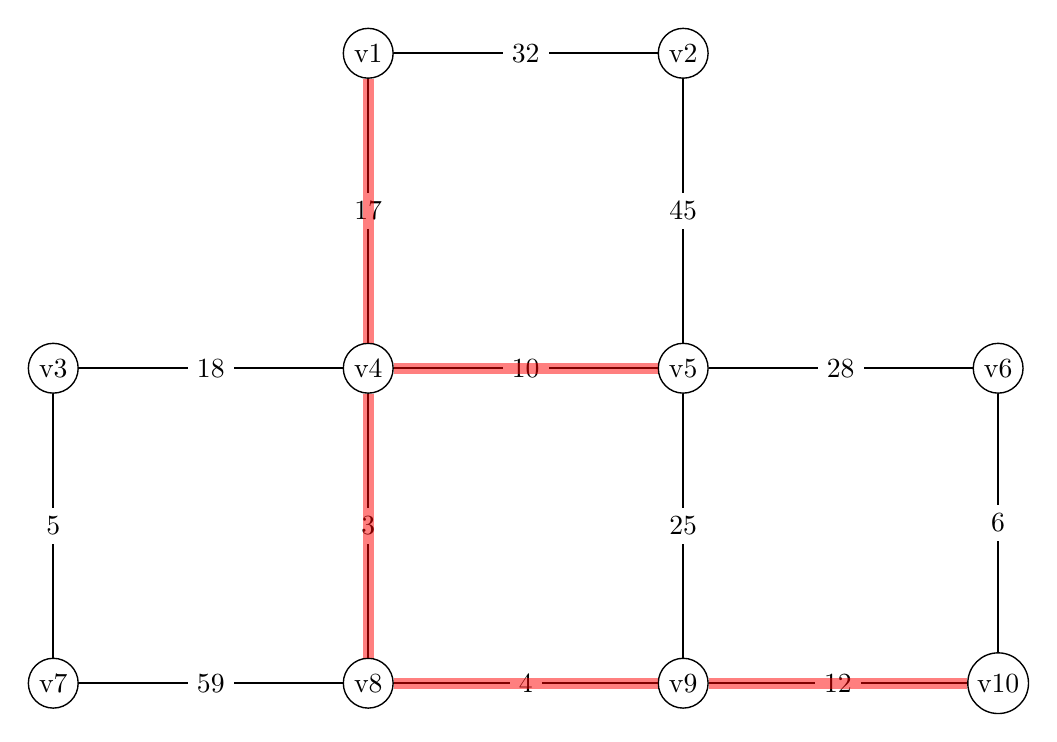
\begin{tikzpicture}
    \GraphInit[vstyle=Dijkstra]
    \SetGraphUnit{4}
    \Vertex{v1}
    \EA(v1){v2}
    \SO(v1){v4}
    \SO(v2){v5}
    \EA(v5){v6}
    \SO(v6){v10}
    \SO(v5){v9}
    \SO(v4){v8}
    \WE(v4){v3}
    \SO(v3){v7}
    
    \Edge[label=$32$](v1)(v2)
    \Edge[label=$17$](v1)(v4)
    \Edge[label=$45$](v2)(v5)
    \Edge[label=$18$](v3)(v4)
    \Edge[label=$10$](v4)(v5)
    \Edge[label=$28$](v6)(v5)
    \Edge[label=$5$](v3)(v7)
    \Edge[label=$3$](v4)(v8)
    \Edge[label=$25$](v5)(v9)
    \Edge[label=$6$](v6)(v10)
    \Edge[label=$59$](v7)(v8)
    \Edge[label=$4$](v8)(v9)
    \Edge[label=$12$](v9)(v10)
    \SetUpEdge[lw=4pt,color=red]
    \Edges[style={opacity=.5}](v1,v4)
    \Edges[style={opacity=.5}](v4,v8)
    \Edges[style={opacity=.5}](v8,v9)
    \Edges[style={opacity=.5}](v4,v5)
    \Edges[style={opacity=.5}](v9,v10)
\end{tikzpicture}

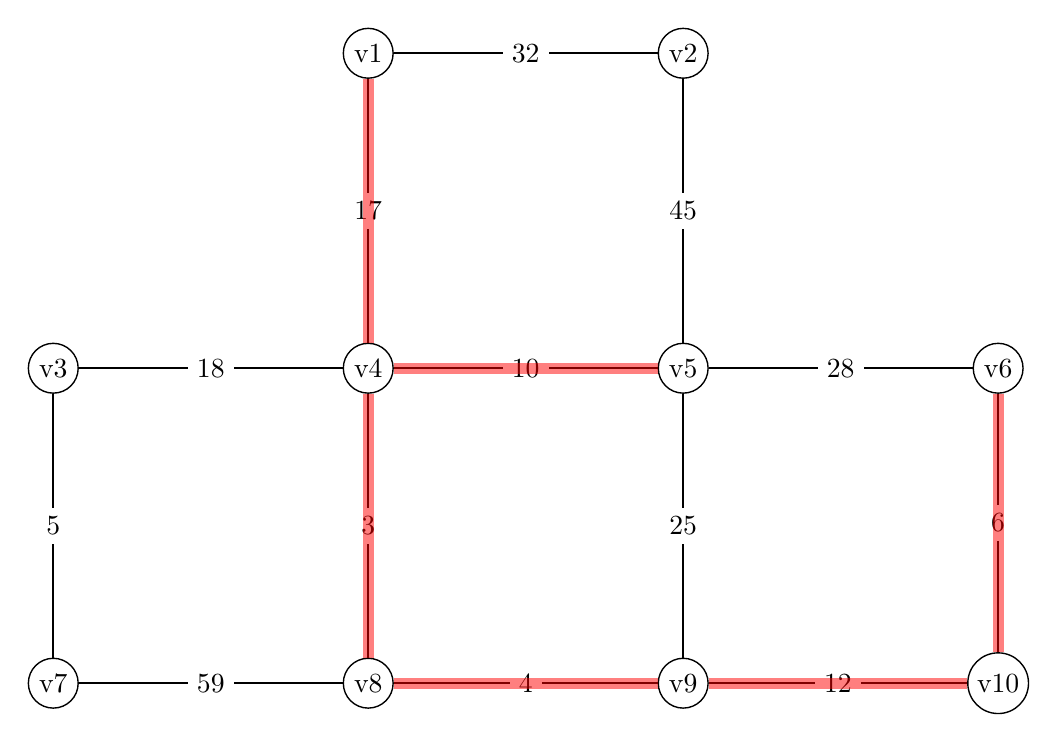
\begin{tikzpicture}
    \GraphInit[vstyle=Dijkstra]
    \SetGraphUnit{4}
    \Vertex{v1}
    \EA(v1){v2}
    \SO(v1){v4}
    \SO(v2){v5}
    \EA(v5){v6}
    \SO(v6){v10}
    \SO(v5){v9}
    \SO(v4){v8}
    \WE(v4){v3}
    \SO(v3){v7}
    
    \Edge[label=$32$](v1)(v2)
    \Edge[label=$17$](v1)(v4)
    \Edge[label=$45$](v2)(v5)
    \Edge[label=$18$](v3)(v4)
    \Edge[label=$10$](v4)(v5)
    \Edge[label=$28$](v6)(v5)
    \Edge[label=$5$](v3)(v7)
    \Edge[label=$3$](v4)(v8)
    \Edge[label=$25$](v5)(v9)
    \Edge[label=$6$](v6)(v10)
    \Edge[label=$59$](v7)(v8)
    \Edge[label=$4$](v8)(v9)
    \Edge[label=$12$](v9)(v10)
    \SetUpEdge[lw=4pt,color=red]
    \Edges[style={opacity=.5}](v1,v4)
    \Edges[style={opacity=.5}](v4,v8)
    \Edges[style={opacity=.5}](v8,v9)
    \Edges[style={opacity=.5}](v4,v5)
    \Edges[style={opacity=.5}](v9,v10)
    \Edges[style={opacity=.5}](v10,v6)
\end{tikzpicture}


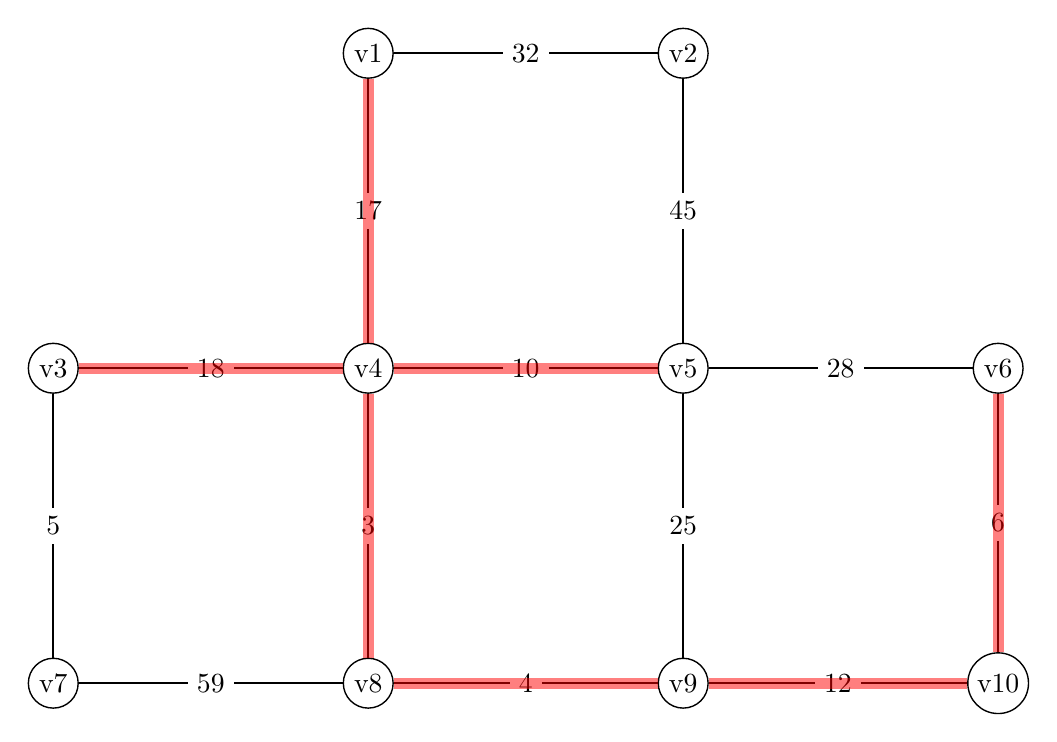
\begin{tikzpicture}
    \GraphInit[vstyle=Dijkstra]
    \SetGraphUnit{4}
    \Vertex{v1}
    \EA(v1){v2}
    \SO(v1){v4}
    \SO(v2){v5}
    \EA(v5){v6}
    \SO(v6){v10}
    \SO(v5){v9}
    \SO(v4){v8}
    \WE(v4){v3}
    \SO(v3){v7}
    
    \Edge[label=$32$](v1)(v2)
    \Edge[label=$17$](v1)(v4)
    \Edge[label=$45$](v2)(v5)
    \Edge[label=$18$](v3)(v4)
    \Edge[label=$10$](v4)(v5)
    \Edge[label=$28$](v6)(v5)
    \Edge[label=$5$](v3)(v7)
    \Edge[label=$3$](v4)(v8)
    \Edge[label=$25$](v5)(v9)
    \Edge[label=$6$](v6)(v10)
    \Edge[label=$59$](v7)(v8)
    \Edge[label=$4$](v8)(v9)
    \Edge[label=$12$](v9)(v10)
    \SetUpEdge[lw=4pt,color=red]
    \Edges[style={opacity=.5}](v1,v4)
    \Edges[style={opacity=.5}](v4,v8)
    \Edges[style={opacity=.5}](v8,v9)
    \Edges[style={opacity=.5}](v4,v5)
    \Edges[style={opacity=.5}](v9,v10)
    \Edges[style={opacity=.5}](v10,v6)
    \Edges[style={opacity=.5}](v4,v3)
\end{tikzpicture}

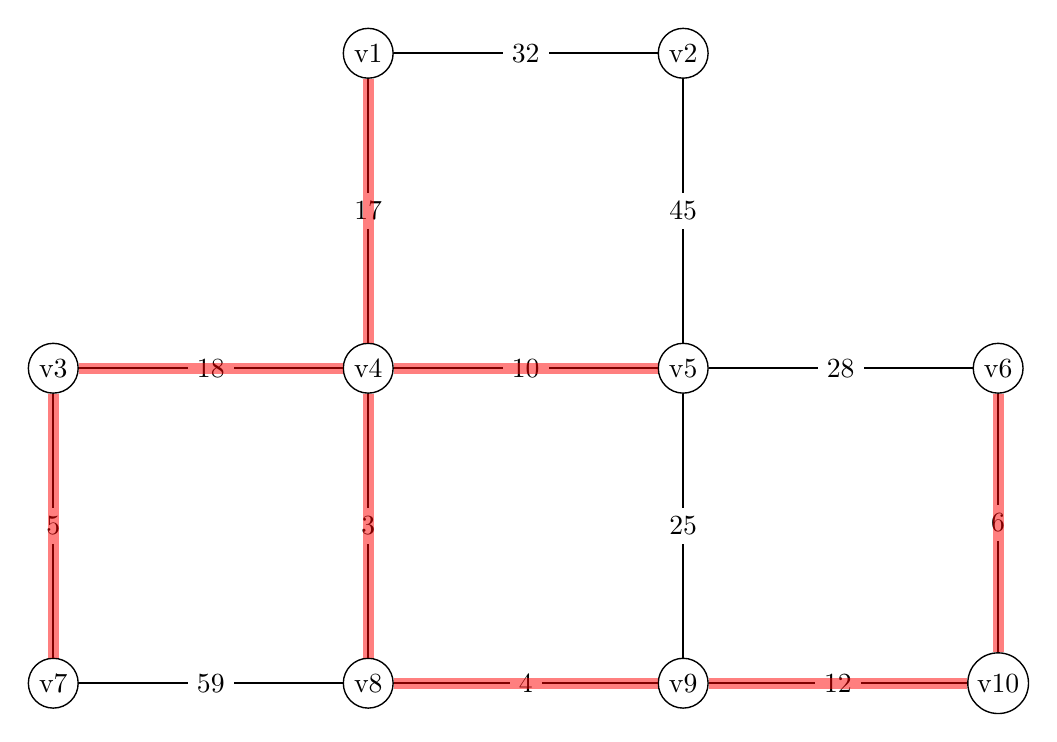
\begin{tikzpicture}
    \GraphInit[vstyle=Dijkstra]
    \SetGraphUnit{4}
    \Vertex{v1}
    \EA(v1){v2}
    \SO(v1){v4}
    \SO(v2){v5}
    \EA(v5){v6}
    \SO(v6){v10}
    \SO(v5){v9}
    \SO(v4){v8}
    \WE(v4){v3}
    \SO(v3){v7}
    
    \Edge[label=$32$](v1)(v2)
    \Edge[label=$17$](v1)(v4)
    \Edge[label=$45$](v2)(v5)
    \Edge[label=$18$](v3)(v4)
    \Edge[label=$10$](v4)(v5)
    \Edge[label=$28$](v6)(v5)
    \Edge[label=$5$](v3)(v7)
    \Edge[label=$3$](v4)(v8)
    \Edge[label=$25$](v5)(v9)
    \Edge[label=$6$](v6)(v10)
    \Edge[label=$59$](v7)(v8)
    \Edge[label=$4$](v8)(v9)
    \Edge[label=$12$](v9)(v10)
    \SetUpEdge[lw=4pt,color=red]
    \Edges[style={opacity=.5}](v1,v4)
    \Edges[style={opacity=.5}](v4,v8)
    \Edges[style={opacity=.5}](v8,v9)
    \Edges[style={opacity=.5}](v4,v5)
    \Edges[style={opacity=.5}](v9,v10)
    \Edges[style={opacity=.5}](v10,v6)
    \Edges[style={opacity=.5}](v4,v3)
    \Edges[style={opacity=.5}](v3,v7)
\end{tikzpicture}

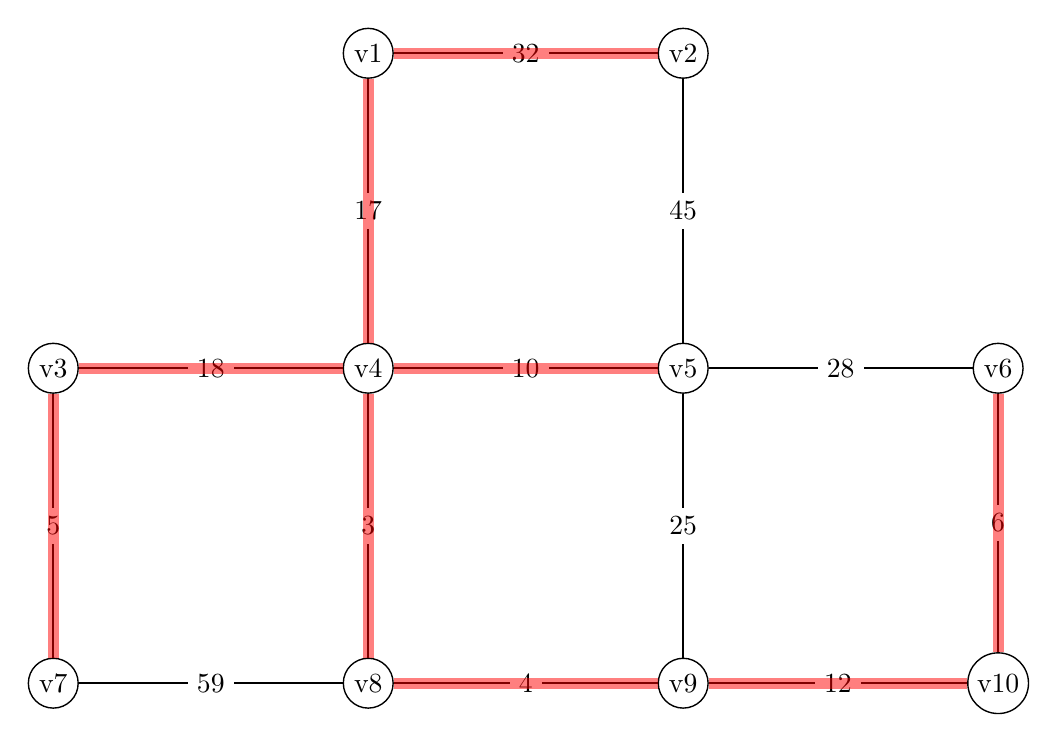
\begin{tikzpicture}
    \GraphInit[vstyle=Dijkstra]
    \SetGraphUnit{4}
    \Vertex{v1}
    \EA(v1){v2}
    \SO(v1){v4}
    \SO(v2){v5}
    \EA(v5){v6}
    \SO(v6){v10}
    \SO(v5){v9}
    \SO(v4){v8}
    \WE(v4){v3}
    \SO(v3){v7}
    
    \Edge[label=$32$](v1)(v2)
    \Edge[label=$17$](v1)(v4)
    \Edge[label=$45$](v2)(v5)
    \Edge[label=$18$](v3)(v4)
    \Edge[label=$10$](v4)(v5)
    \Edge[label=$28$](v6)(v5)
    \Edge[label=$5$](v3)(v7)
    \Edge[label=$3$](v4)(v8)
    \Edge[label=$25$](v5)(v9)
    \Edge[label=$6$](v6)(v10)
    \Edge[label=$59$](v7)(v8)
    \Edge[label=$4$](v8)(v9)
    \Edge[label=$12$](v9)(v10)
    \SetUpEdge[lw=4pt,color=red]
    \Edges[style={opacity=.5}](v1,v4)
    \Edges[style={opacity=.5}](v4,v8)
    \Edges[style={opacity=.5}](v8,v9)
    \Edges[style={opacity=.5}](v4,v5)
    \Edges[style={opacity=.5}](v9,v10)
    \Edges[style={opacity=.5}](v10,v6)
    \Edges[style={opacity=.5}](v4,v3)
    \Edges[style={opacity=.5}](v3,v7)
    \Edges[style={opacity=.5}](v1,v2)
\end{tikzpicture}


\end{solutionorbox}

\ifprintanswers
\newpage
\else
\bigskip
\fi
	
	
%%%%%%%%%%%%%%%%%%%%%%%%%%%%%%%%%%%%%%%%%%%%%%%%%%%%%%%%%%%%%%%%%%
% Question
%%%%%%%%%%%%%%%%%%%%%%%%%%%%%%%%%%%%%%%%%%%%%%%%%%%%%%%%%%%%%%%%%%
\question[10]
Use Kruskal's algorithm to find a minimum spanning tree for the graph shown above.  Show the actions step by step.
\begin{solutionorbox}
	
Hoàng Thông Trương
2:46 PM (9 minutes ago)
to me

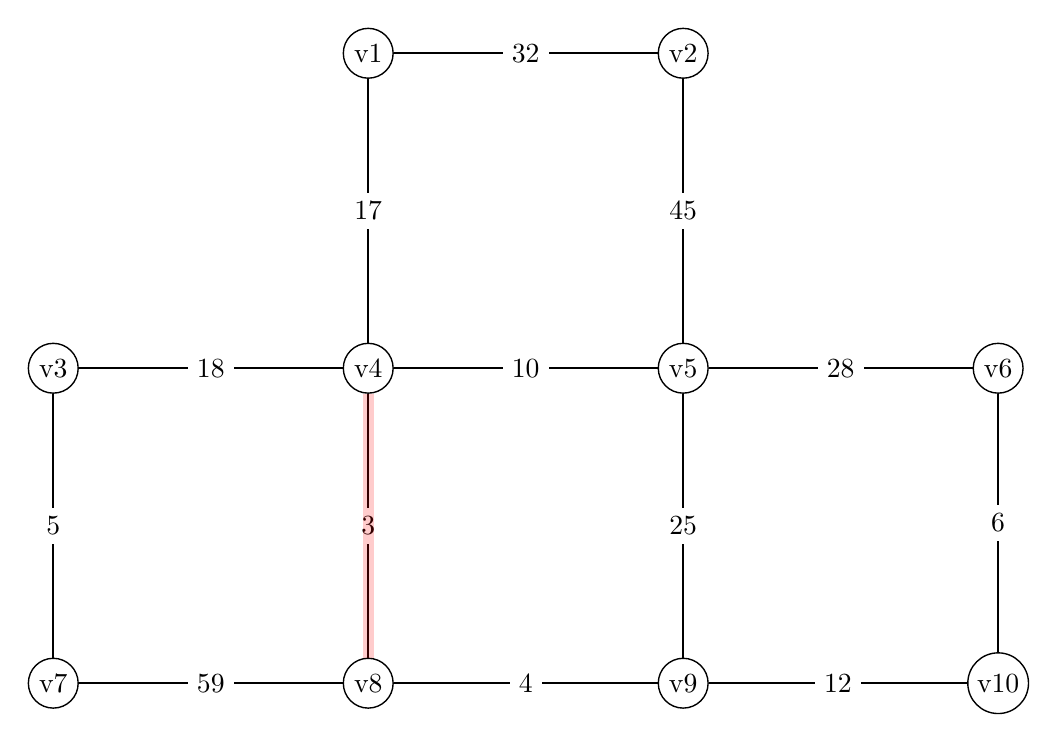
\begin{tikzpicture}
    \GraphInit[vstyle=Dijkstra]
    \SetGraphUnit{4}
    \Vertex{v1}
    \EA(v1){v2}
    \SO(v1){v4}
    \SO(v2){v5}
    \EA(v5){v6}
    \SO(v6){v10}
    \SO(v5){v9}
    \SO(v4){v8}
    \WE(v4){v3}
    \SO(v3){v7}
   
    \Edge[label=$32$](v1)(v2)
    \Edge[label=$17$](v1)(v4)
    \Edge[label=$45$](v2)(v5)
    \Edge[label=$18$](v3)(v4)
    \Edge[label=$10$](v4)(v5)
    \Edge[label=$28$](v6)(v5)
    \Edge[label=$5$](v3)(v7)
    \Edge[label=$3$](v4)(v8)
    \Edge[label=$25$](v5)(v9)
    \Edge[label=$6$](v6)(v10)
    \Edge[label=$59$](v7)(v8)
    \Edge[label=$4$](v8)(v9)
    \Edge[label=$12$](v9)(v10)
    \SetUpEdge[lw=4pt,color=red]
    \Edges[style={opacity=.2}](v4,v8)
\end{tikzpicture}

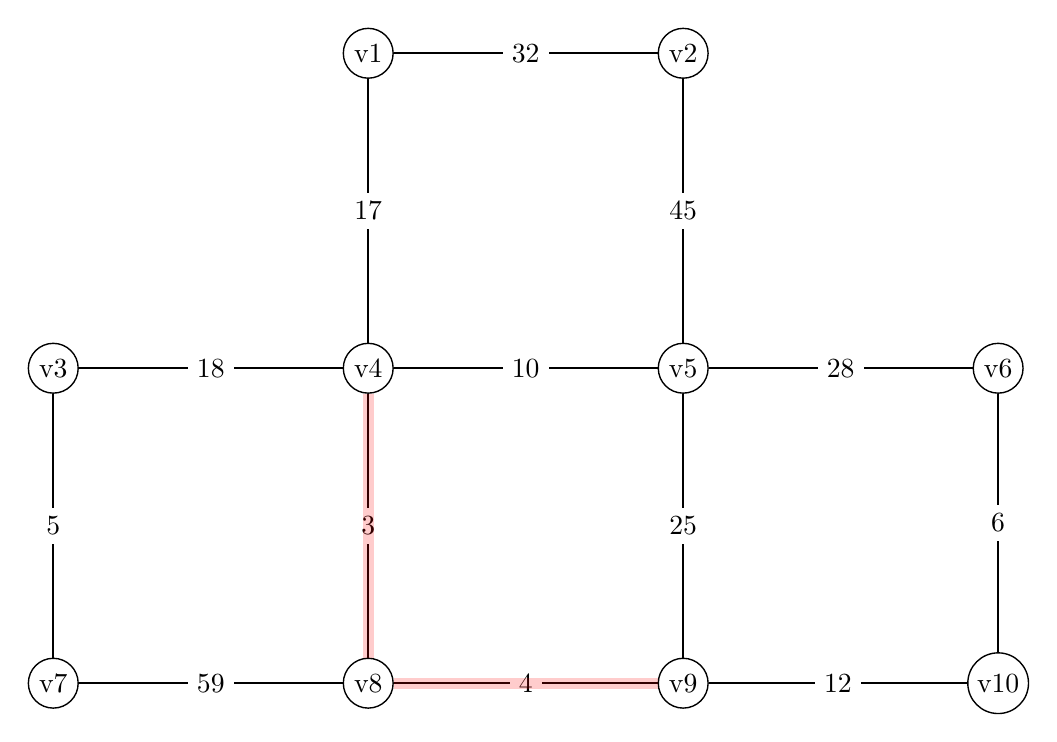
\begin{tikzpicture}
    \GraphInit[vstyle=Dijkstra]
    \SetGraphUnit{4}
    \Vertex{v1}
    \EA(v1){v2}
    \SO(v1){v4}
    \SO(v2){v5}
    \EA(v5){v6}
    \SO(v6){v10}
    \SO(v5){v9}
    \SO(v4){v8}
    \WE(v4){v3}
    \SO(v3){v7}
   
    \Edge[label=$32$](v1)(v2)
    \Edge[label=$17$](v1)(v4)
    \Edge[label=$45$](v2)(v5)
    \Edge[label=$18$](v3)(v4)
    \Edge[label=$10$](v4)(v5)
    \Edge[label=$28$](v6)(v5)
    \Edge[label=$5$](v3)(v7)
    \Edge[label=$3$](v4)(v8)
    \Edge[label=$25$](v5)(v9)
    \Edge[label=$6$](v6)(v10)
    \Edge[label=$59$](v7)(v8)
    \Edge[label=$4$](v8)(v9)
    \Edge[label=$12$](v9)(v10)
    \SetUpEdge[lw=4pt,color=red]
    \Edges[style={opacity=.2}](v4,v8,v9)
\end{tikzpicture}

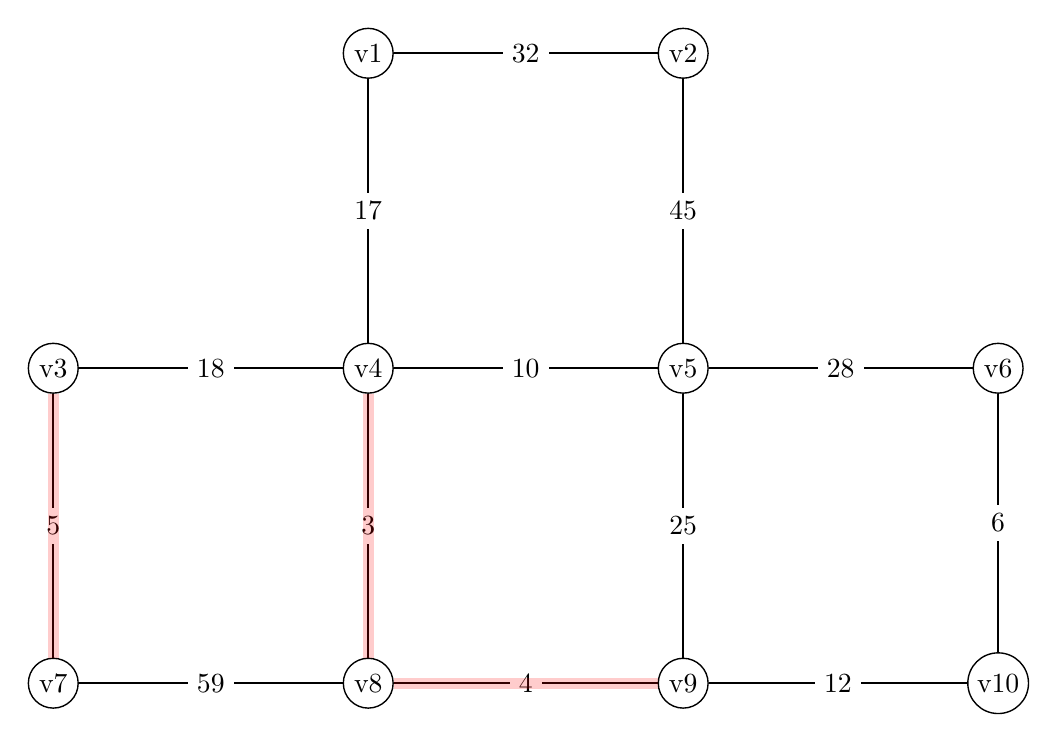
\begin{tikzpicture}
    \GraphInit[vstyle=Dijkstra]
    \SetGraphUnit{4}
    \Vertex{v1}
    \EA(v1){v2}
    \SO(v1){v4}
    \SO(v2){v5}
    \EA(v5){v6}
    \SO(v6){v10}
    \SO(v5){v9}
    \SO(v4){v8}
    \WE(v4){v3}
    \SO(v3){v7}
   
    \Edge[label=$32$](v1)(v2)
    \Edge[label=$17$](v1)(v4)
    \Edge[label=$45$](v2)(v5)
    \Edge[label=$18$](v3)(v4)
    \Edge[label=$10$](v4)(v5)
    \Edge[label=$28$](v6)(v5)
    \Edge[label=$5$](v3)(v7)
    \Edge[label=$3$](v4)(v8)
    \Edge[label=$25$](v5)(v9)
    \Edge[label=$6$](v6)(v10)
    \Edge[label=$59$](v7)(v8)
    \Edge[label=$4$](v8)(v9)
    \Edge[label=$12$](v9)(v10)
    \SetUpEdge[lw=4pt,color=red]
    \Edges[style={opacity=.2}](v4,v8,v9)
    \Edges[style={opacity=.2}](v3,v7)
\end{tikzpicture}

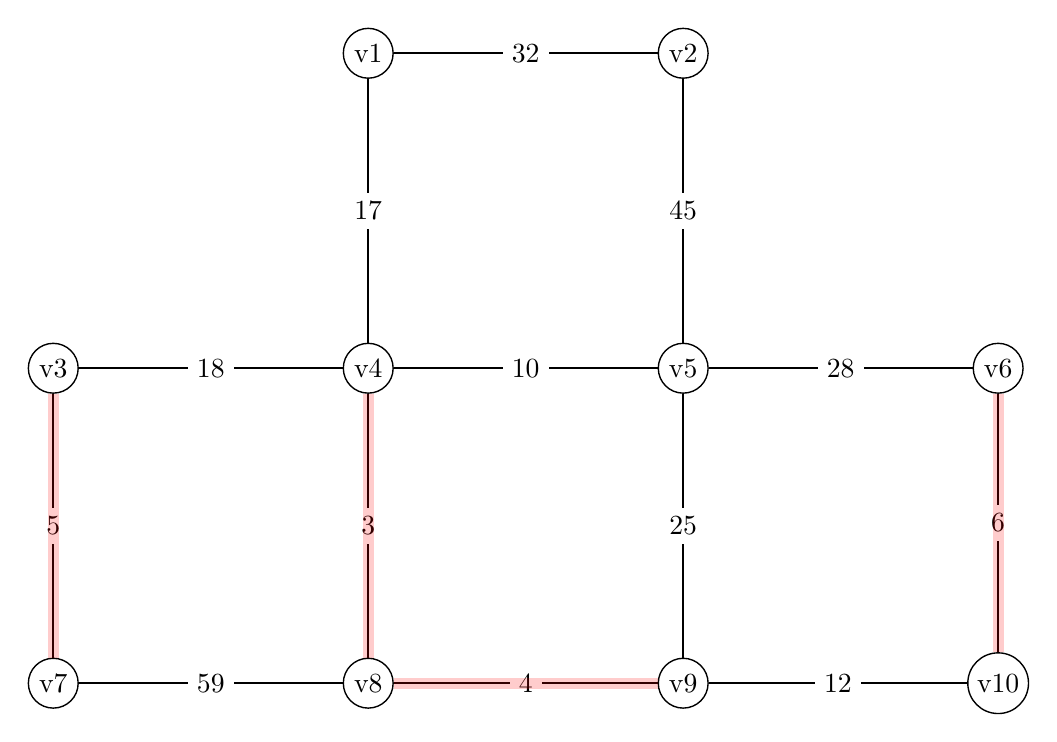
\begin{tikzpicture}
    \GraphInit[vstyle=Dijkstra]
    \SetGraphUnit{4}
    \Vertex{v1}
    \EA(v1){v2}
    \SO(v1){v4}
    \SO(v2){v5}
    \EA(v5){v6}
    \SO(v6){v10}
    \SO(v5){v9}
    \SO(v4){v8}
    \WE(v4){v3}
    \SO(v3){v7}
   
    \Edge[label=$32$](v1)(v2)
    \Edge[label=$17$](v1)(v4)
    \Edge[label=$45$](v2)(v5)
    \Edge[label=$18$](v3)(v4)
    \Edge[label=$10$](v4)(v5)
    \Edge[label=$28$](v6)(v5)
    \Edge[label=$5$](v3)(v7)
    \Edge[label=$3$](v4)(v8)
    \Edge[label=$25$](v5)(v9)
    \Edge[label=$6$](v6)(v10)
    \Edge[label=$59$](v7)(v8)
    \Edge[label=$4$](v8)(v9)
    \Edge[label=$12$](v9)(v10)
    \SetUpEdge[lw=4pt,color=red]
    \Edges[style={opacity=.2}](v4,v8,v9)
    \Edges[style={opacity=.2}](v3,v7)
    \Edges[style={opacity=.2}](v6,v10)
\end{tikzpicture}

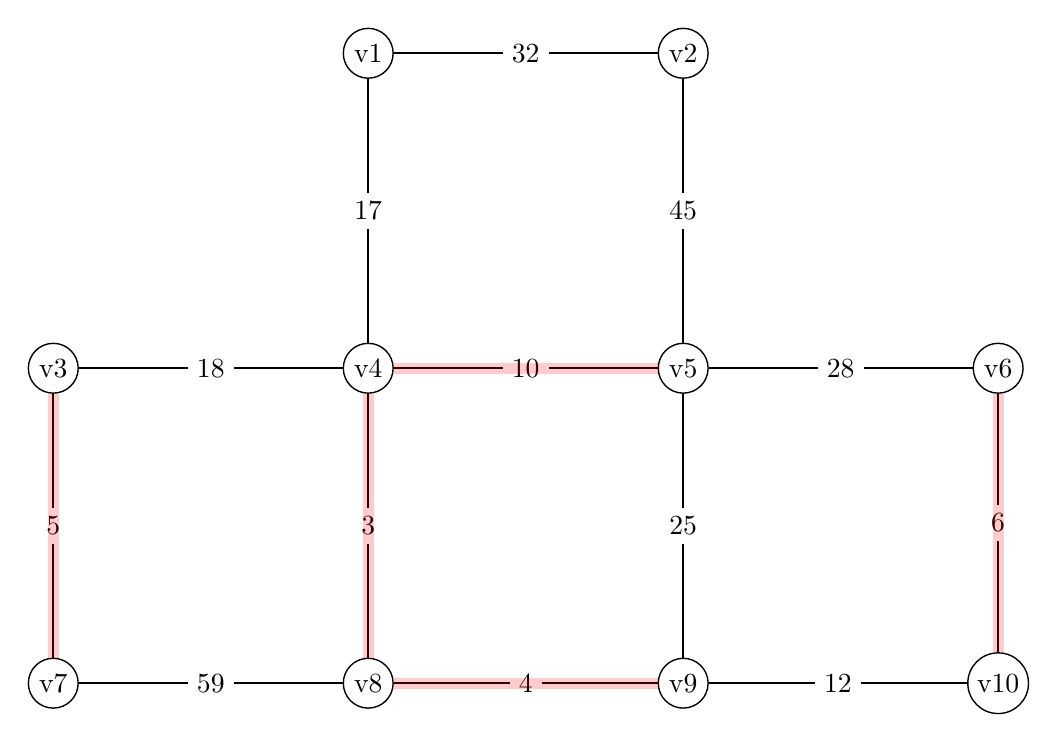
\begin{tikzpicture}
    \GraphInit[vstyle=Dijkstra]
    \SetGraphUnit{4}
    \Vertex{v1}
    \EA(v1){v2}
    \SO(v1){v4}
    \SO(v2){v5}
    \EA(v5){v6}
    \SO(v6){v10}
    \SO(v5){v9}
    \SO(v4){v8}
    \WE(v4){v3}
    \SO(v3){v7}
   
    \Edge[label=$32$](v1)(v2)
    \Edge[label=$17$](v1)(v4)
    \Edge[label=$45$](v2)(v5)
    \Edge[label=$18$](v3)(v4)
    \Edge[label=$10$](v4)(v5)
    \Edge[label=$28$](v6)(v5)
    \Edge[label=$5$](v3)(v7)
    \Edge[label=$3$](v4)(v8)
    \Edge[label=$25$](v5)(v9)
    \Edge[label=$6$](v6)(v10)
    \Edge[label=$59$](v7)(v8)
    \Edge[label=$4$](v8)(v9)
    \Edge[label=$12$](v9)(v10)
    \SetUpEdge[lw=4pt,color=red]
    \Edges[style={opacity=.2}](v4,v8,v9)
    \Edges[style={opacity=.2}](v3,v7)
    \Edges[style={opacity=.2}](v6,v10)
    \Edges[style={opacity=.2}](v4,v5)
\end{tikzpicture}

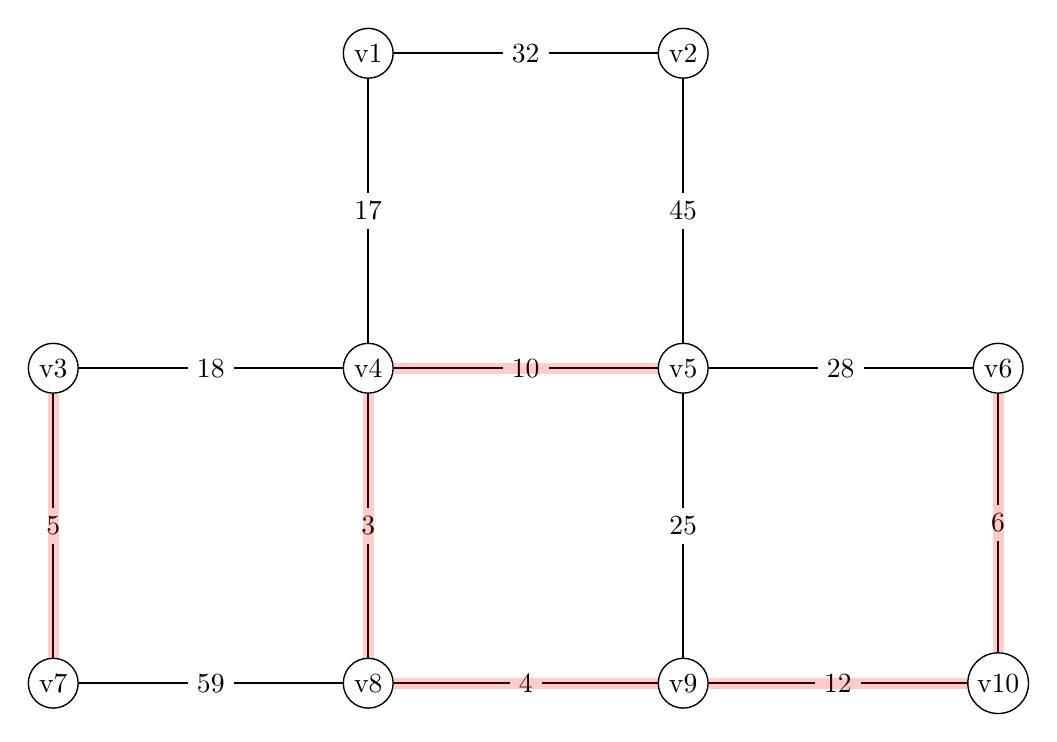
\begin{tikzpicture}
    \GraphInit[vstyle=Dijkstra]
    \SetGraphUnit{4}
    \Vertex{v1}
    \EA(v1){v2}
    \SO(v1){v4}
    \SO(v2){v5}
    \EA(v5){v6}
    \SO(v6){v10}
    \SO(v5){v9}
    \SO(v4){v8}
    \WE(v4){v3}
    \SO(v3){v7}
   
    \Edge[label=$32$](v1)(v2)
    \Edge[label=$17$](v1)(v4)
    \Edge[label=$45$](v2)(v5)
    \Edge[label=$18$](v3)(v4)
    \Edge[label=$10$](v4)(v5)
    \Edge[label=$28$](v6)(v5)
    \Edge[label=$5$](v3)(v7)
    \Edge[label=$3$](v4)(v8)
    \Edge[label=$25$](v5)(v9)
    \Edge[label=$6$](v6)(v10)
    \Edge[label=$59$](v7)(v8)
    \Edge[label=$4$](v8)(v9)
    \Edge[label=$12$](v9)(v10)
    \SetUpEdge[lw=4pt,color=red]
    \Edges[style={opacity=.2}](v4,v8,v9,v10)
    \Edges[style={opacity=.2}](v3,v7)
    \Edges[style={opacity=.2}](v6,v10)
    \Edges[style={opacity=.2}](v4,v5)
   
\end{tikzpicture}

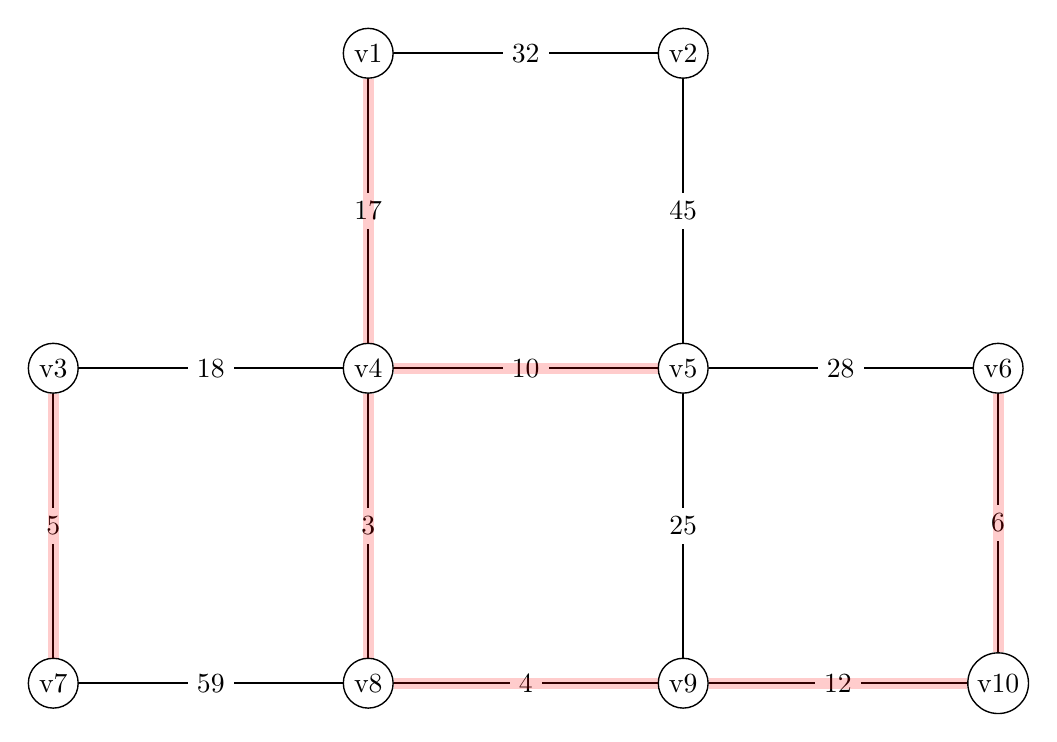
\begin{tikzpicture}
    \GraphInit[vstyle=Dijkstra]
    \SetGraphUnit{4}
    \Vertex{v1}
    \EA(v1){v2}
    \SO(v1){v4}
    \SO(v2){v5}
    \EA(v5){v6}
    \SO(v6){v10}
    \SO(v5){v9}
    \SO(v4){v8}
    \WE(v4){v3}
    \SO(v3){v7}
   
    \Edge[label=$32$](v1)(v2)
    \Edge[label=$17$](v1)(v4)
    \Edge[label=$45$](v2)(v5)
    \Edge[label=$18$](v3)(v4)
    \Edge[label=$10$](v4)(v5)
    \Edge[label=$28$](v6)(v5)
    \Edge[label=$5$](v3)(v7)
    \Edge[label=$3$](v4)(v8)
    \Edge[label=$25$](v5)(v9)
    \Edge[label=$6$](v6)(v10)
    \Edge[label=$59$](v7)(v8)
    \Edge[label=$4$](v8)(v9)
    \Edge[label=$12$](v9)(v10)
    \SetUpEdge[lw=4pt,color=red]
    \Edges[style={opacity=.2}](v4,v8,v9,v10)
    \Edges[style={opacity=.2}](v3,v7)
    \Edges[style={opacity=.2}](v6,v10)
    \Edges[style={opacity=.2}](v4,v5)
    \Edges[style={opacity=.2}](v1,v4)
\end{tikzpicture}

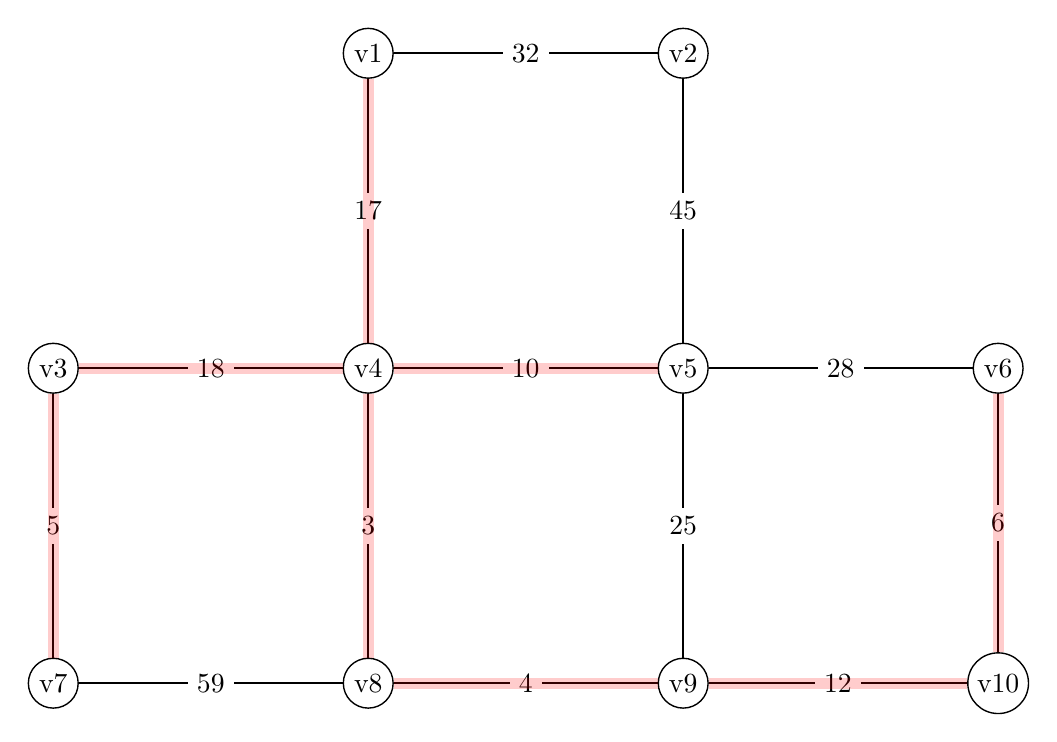
\begin{tikzpicture}
    \GraphInit[vstyle=Dijkstra]
    \SetGraphUnit{4}
    \Vertex{v1}
    \EA(v1){v2}
    \SO(v1){v4}
    \SO(v2){v5}
    \EA(v5){v6}
    \SO(v6){v10}
    \SO(v5){v9}
    \SO(v4){v8}
    \WE(v4){v3}
    \SO(v3){v7}
   
    \Edge[label=$32$](v1)(v2)
    \Edge[label=$17$](v1)(v4)
    \Edge[label=$45$](v2)(v5)
    \Edge[label=$18$](v3)(v4)
    \Edge[label=$10$](v4)(v5)
    \Edge[label=$28$](v6)(v5)
    \Edge[label=$5$](v3)(v7)
    \Edge[label=$3$](v4)(v8)
    \Edge[label=$25$](v5)(v9)
    \Edge[label=$6$](v6)(v10)
    \Edge[label=$59$](v7)(v8)
    \Edge[label=$4$](v8)(v9)
    \Edge[label=$12$](v9)(v10)
    \SetUpEdge[lw=4pt,color=red]
    \Edges[style={opacity=.2}](v4,v8,v9,v10)
    \Edges[style={opacity=.2}](v3,v7)
    \Edges[style={opacity=.2}](v6,v10)
    \Edges[style={opacity=.2}](v4,v5)
    \Edges[style={opacity=.2}](v1,v4,v3)
\end{tikzpicture}

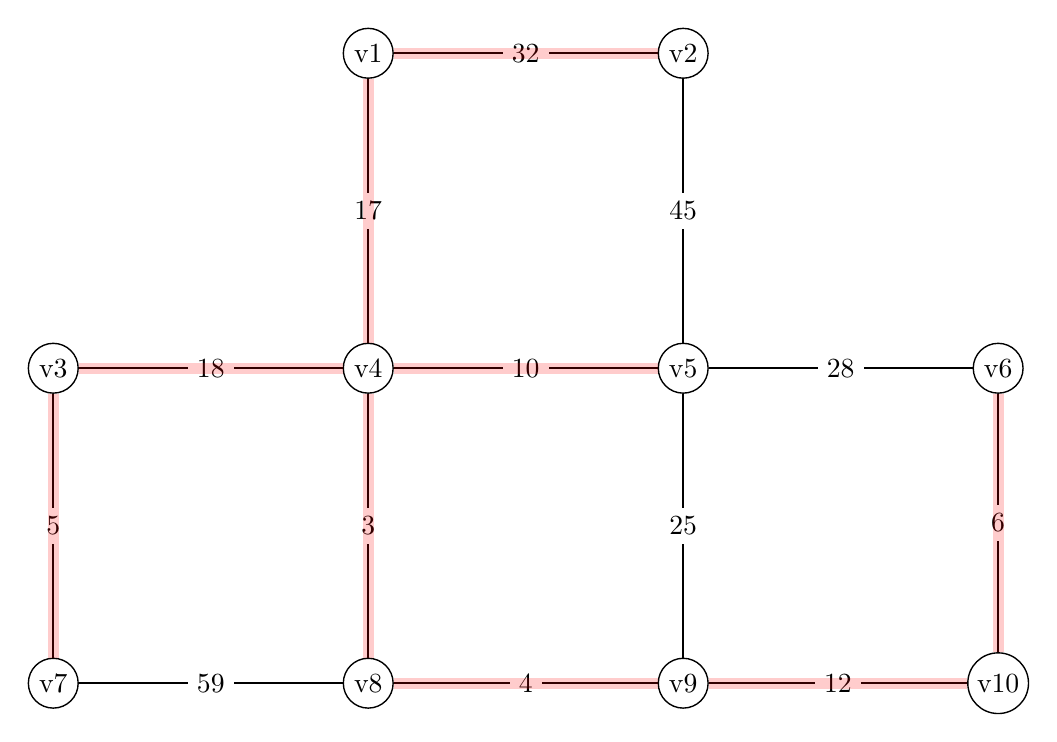
\begin{tikzpicture}
    \GraphInit[vstyle=Dijkstra]
    \SetGraphUnit{4}
    \Vertex{v1}
    \EA(v1){v2}
    \SO(v1){v4}
    \SO(v2){v5}
    \EA(v5){v6}
    \SO(v6){v10}
    \SO(v5){v9}
    \SO(v4){v8}
    \WE(v4){v3}
    \SO(v3){v7}
   
    \Edge[label=$32$](v1)(v2)
    \Edge[label=$17$](v1)(v4)
    \Edge[label=$45$](v2)(v5)
    \Edge[label=$18$](v3)(v4)
    \Edge[label=$10$](v4)(v5)
    \Edge[label=$28$](v6)(v5)
    \Edge[label=$5$](v3)(v7)
    \Edge[label=$3$](v4)(v8)
    \Edge[label=$25$](v5)(v9)
    \Edge[label=$6$](v6)(v10)
    \Edge[label=$59$](v7)(v8)
    \Edge[label=$4$](v8)(v9)
    \Edge[label=$12$](v9)(v10)
    \SetUpEdge[lw=4pt,color=red]
    \Edges[style={opacity=.2}](v4,v8,v9,v10)
    \Edges[style={opacity=.2}](v3,v7)
    \Edges[style={opacity=.2}](v6,v10)
    \Edges[style={opacity=.2}](v4,v5)
    \Edges[style={opacity=.2}](v1,v4,v3)
    \Edges[style={opacity=.2}](v1,v2)
\end{tikzpicture}
\end{solutionorbox}

\ifprintanswers
\newpage
\else
\bigskip
\fi
	
	
%%%%%%%%%%%%%%%%%%%%%%%%%%%%%%%%%%%%%%%%%%%%%%%%%%%%%%%%%%%%%%%%%%
% Question
%%%%%%%%%%%%%%%%%%%%%%%%%%%%%%%%%%%%%%%%%%%%%%%%%%%%%%%%%%%%%%%%%%
\question[5]  True or False, and justify.  If true, show why the statement is correct.  If false, show why the statement is incorrect and show the correct answer.
\begin{center}
	\textit{It is possible for a minimum spanning tree to have a cycle.}
\end{center}
\begin{solutionorbox}
	False. A minimum spanning tree, by definition, has the minimum number of edges required to reach all vertices. Therefore it cannot have a cycle since for any cycle you can remove at least one edge and have it reach all the vertices. Therefore the correct answer would be \emph{It is impossible for a MST to have a cycle}
\end{solutionorbox}

\ifprintanswers
\newpage
\else
\bigskip
\fi


%%%%%%%%%%%%%%%%%%%%%%%%%%%%%%%%%%%%%%%%%%%%%%%%%%%%%%%%%%%%%%%%%%
% Question
%%%%%%%%%%%%%%%%%%%%%%%%%%%%%%%%%%%%%%%%%%%%%%%%%%%%%%%%%%%%%%%%%%
\question [5] Assume that in a network of computers any two computers can be linked.  Given a cost estimate for each possible link, should Prim's algorithm or Kruskal's algorithm be used?  Justify your answer.
\begin{solutionorbox}
    I would use Prim's Algorithm. Since any 2 computers can be linked, then that means that the tree is dense, since everything is together. Prims algorithm is faster for a dense tree. 
\end{solutionorbox}

\ifprintanswers
\newpage
\else
\bigskip
\fi


%%%%%%%%%%%%%%%%%%%%%%%%%%%%%%%%%%%%%%%%%%%%%%%%%%%%%%%%%%%%%%%%%%
% Question
%%%%%%%%%%%%%%%%%%%%%%%%%%%%%%%%%%%%%%%%%%%%%%%%%%%%%%%%%%%%%%%%%%
\question [10] Problem 23.2-2.  Suppose that we represent the graph $G=(V,E)$ as an adjacency matrix.  Give a simple implementation of Prim's algorithm for this case that runs in $O(V^2)$ time.
\begin{solutionorbox}
	    \begin{minted}{python}
import numpy as np
#adapted from class notes but slightly different
#NOTE: G in this case is an adjecency matrix
#output in the case is in the format "Edge : Weight" 
def Prim(G, Size):
    selected_node = [0] * Size

    no_edge = 0

    selected_node[0] = True

    while (no_edge < N - 1):
    
    minimum = np.inf
    a = 0
    b = 0
    for m in range(Size):
        if selected_node[m]:
            for n in range(Size):
                if ((not selected_node[n]) and G[m][n]):  
                    # not in selected and there is an edge
                    if minimum > G[m][n]:
                        minimum = G[m][n]
                        a = m
                        b = n
    print(str(a) + "-" + str(b) + ":" + str(G[a][b]))
    selected_node[b] = True
    no_edge += 1
\end{minted}
\end{solutionorbox}

%\ifprintanswers
%\newpage
%\else
%\bigskip
%\fi

%%%%%%%%%%%%%%%%%%%%%%%%%%%%%%%%%%%%%%%%%%%%%%%%%%%%%%%%%%%%%%%%%%
%%%%%%%%%%%%%%%%%%%%%%%%%%%%%%%%%%%%%%%%%%%%%%%%%%%%%%%%%%%%%%%%%%
\end{questions}
\end{document}
